\section{Advanced C++}

\subsection{Static vs. Dynamic Binding}
\begin{itemize}
	\item Static binding (early binding, statische Bindung)
		\begin{itemize}
			\item Bereits zur Compilezeit wird festgelegt, welcher (Elementfunktions-) Code
				ausgeführt wird (Normalfall)
			\item ''Normale`` Klassen, templates
		\end{itemize}
	\item Dynamic binding (late binding, dynamische Bindung)
		\begin{itemize}
			\item Erst zur Laufzeit wird in Abhängigkeit des Objekts festgelegt, welcher
				(Elementfunktions-) Code ausgeführt wird
			\item Run-Time Polymorphismus, virtual
			\item Laufzeit mehraufwand, weniger effizient
		\end{itemize}
\end{itemize}

\subsubsection{Virtuelle Memberfunktionen (Siehe Zf\_OOProg)}
Soll die Funktion überschrieben werden können, muss \emph{virtual} verwendet werden.
Wird virtual nicht verwendet, wird die Funktion nur ''versteckt``.
\lstinputlisting{code/virttest.cpp}


\subsection[RAII]{RAII - RESOURCE ACQUISITION IS INITIALISATION}

\paragraph{Motivation}
Resourcen (Datei, Speicher, Semaphoren) müssen vor Gebrauch angefordert und danach wieder freigegeben werden.
Dazwischen könnte aber z.B. eine Exception auftreten, was das Freigeben verhindert.

\paragraph{Lösung}
Damit die Resource trotzdem freigegeben wird, kann sie als Klassen-Objekt instanziert werden. Das Objekt wird automatisch gelöscht wenn es seine Gültigkeit (out-of-scope) verliert.
\begin{compactitem}
	\item Konstruktor fordert die Resource an
	\item Destruktor gibt sie wieder frei
\end{compactitem}


\paragraph{Heap-Objekte}
Für Heap-Objekte stellt die Boost-Library Templates für diesen Zweck zur Verfügung.\\
Problem:
\begin{lstlisting}
void f()
{
	Person* p = new Person("irgendwer");
	// mach etwas mit p
	// was ist, wenn vorher eine Exception geworfen wird?
	delete p;
}
\end{lstlisting}

Lösung:
\begin{lstlisting}
void f()
{
	boost::shared_ptr<Person> p(new Person("irgendwer"));
	// mach etwas mit p
	// Beim Verlassen des Blocks räumt Destruktor von shared_ptr
	// automatisch auf und löscht die Person
}
\end{lstlisting}


\paragraph{Semaphoren} Für Semaphoren könnte die folgende Implementierung verwendet werden


\begin{lstlisting}
class Semaphore
{
public:
	Semaphore(int s=0): id(s) {getSem(s);}
	~Semaphore() {releaseSem(id);}
private:
	int id;
};
\end{lstlisting}
\begin{lstlisting}
void f()
{
  // kritischer Abschnitt
  {
    Semaphore myS; 
  } // hier wird Semaphore freigegeben, Destruktor wird aufgerufen
}
\end{lstlisting}


\subsection[pImpl]{pImpl - \textcolor{red}{P}ointer to \textcolor{red}{Impl}ementation}
\label{sec:pimpl}

\paragraph{Problem} Wie kann man die Implementierung einer Klasse so verstecken, dass man sie
ändern kann, ohne alle Module, welche die Klasse nutzen, bei einer Änderung
neu übersetzen zu müssen?
Nützlich zum Beispiel für eine shared library / DLL.

\paragraph{Lösung}
\begin{itemize}
\item Implementierung im .cpp File wird in einem separatem File versteckt
\item Im Header nur noch die öffentliche Schnittstelle mit einem Pointer auf die Implementierung
\item Die Implementation wird auf dem Heap angelegt $\rightarrow$ unproblematisch weil diese Objekt beim Programmstart angelegt und erst am Schluss wieder freigegeben wird
\end{itemize}

\begin{lstlisting}
#ifndef HIDDENCOUNTER_H_ // public file
#define HIDDENCOUNTER_H_
#include <boost/shared_ptr.hpp>
class HiddenCounter
{
public:
	HiddenCounter(int i=0);
	void inc();
	int count() const;
	void reset();
private:
	boost::shared_ptr<class CounterImpl> pImpl;
};
#endif // HIDDENCOUNTER_H_

#include "HiddenCounter.h" // private file
class CounterImpl
{
public:
	CounterImpl(int i): counter(i) {}
	void inc() { ++counter; }
	int count() const { return counter;}
	void reset() { counter=0; }
private:
	int counter;
};
HiddenCounter::HiddenCounter(int i)
:pImpl(new CounterImpl(i)) {}
void HiddenCounter::inc() {pImpl->inc();}
int HiddenCounter::count() const
	{ return pImpl->count(); }
void HiddenCounter::reset() {pImpl->reset();}
\end{lstlisting}


\subsection{Performance}

\subsubsection{Variablen}
\begin{itemize}
	\item Wenn möglich immer Standardtypen verwenden (int, unsigned int), da
		diese den Registerbreiten entsprechen
	\item Typen wie short und char sparen kaum Platz und sind meistens
		langsamer, da sie speziell behandelt werden müssen.
	\item Werden definierte Bitlängen benötigt (Portabilität), sollten die Typen aus
		$<inttypes.h>$ bzw. $<stdint.h>$ (ab C99): 
		intN\_t,  uintN\_t z.b. uint8\_t \\
		Sie können auch selbst getypedeft werden.
\end{itemize}

Lokale Variablen sollte man so verwenden, dass sie in Registern gebraucht werden können.
Z.b. verhindern Pointer auf lokale Variablen, dass diese in ein Register gelegt werden.

\subsubsection{Lächerliches}
++i soll angeblich schneller sein als i++, da aber i++ viel hübscher aussieht sollte man es eher verwenden ;)\\
PostFix Operatoren benötigen einen Tmp Variable. Gute Compiler werden diese weg optimieren.

\subsection{C++ vs. C}
\begin{itemize}
	\item No-Cost C++ features
		\begin{itemize}
			\item Klassen
			\item Namespaces
			\item Statische Funktionen und Daten
			\item Nicht virtuelle Funktionen
			\item Überladung
			\item Default Parameter, es ist aber zu beachten, dass diese immer übergeben werden, bei grossen Objekten ist dies ineffizient:
				\begin{lstlisting}
void doThat(const std\dotsstring& name = "Unnamed"); // Bad
const std\dotsstring defaultName = "Unnamed";
void doThat(const std\dotsstring& name = defaultName); // Better
				\end{lstlisting}
			\item  Konstruktoren / Destruktoren, sofern korrekt verwendet
			\item Einfache Vererbung
		\end{itemize}
	\item Low-Cost C++ features
		\begin{itemize}
			\item Exceptions, jedoch kann anderes Error-Handling, z.B. via return values auch teuer sein.
		\end{itemize}
	\item High-Cost C++ features, wenn falsch verwendet
		\begin{itemize}
			\item Temporäre Objekte, Objektkopieen (z.B. gibt a+b ein temporäres Objekt zurück), kann einfach vermieden werden
			\item Templates können zu Code-Bloat führen (Bei richtiger Anwendung kann man aber die Performance steigern)
		\end{itemize}
	\item Vorteil von C++
    	\begin{itemize}
	        \item Abstraktion
	        \item Entkapselung
	        \item Inline Operationen
	        \item Shift work from runtime to compile-time
    	\end{itemize}
\end{itemize}


\subsection{Inlining}
\begin{itemize}
	\item Vorteile
		\begin{itemize}
			\item Kein Funktionsaufruf (kein Overhead)
			\item Daher schneller
		\end{itemize}
	\item Nachteile
		\begin{itemize}
			\item Mehr Code
			\item Schwerer zu debuggen
		\end{itemize}
	\item Beschränkungen
		\begin{itemize}
			\item Compiler kann inlining ignorieren
			\item Inlining unmöglich für:
				\begin{itemize}
					\item Funktionen auf die ein Pointer zeigt
					\item Virtuelle Funktionen
					\item Rekursive Funktionen
				\end{itemize}
			\item Linker kann selten Inlinen, daher inlinefunktionen im Header definieren.

		\end{itemize}
\end{itemize}
Implizit / Explizit Inline
\begin{lstlisting}
//example.h
void mf1() { ... }  // implizit inline
inline void mf2() { ... }  // explizit inline
\end{lstlisting}

\subsection{Polymorphismus}
\begin{itemize}
	\item Runtime
		\begin{itemize}
			\item Vererbung, virtuelle Funktionen
			\item Am flexibelsten, kann Informationen verwenden die erst zur Laufzeit bekannt sind
			\item Teurer Laufzeitaufwand, vptrs, vtpls, alles non-inline
		\end{itemize}
	\item Link-Time
		\begin{itemize}
			\item Separat kompilierte Funktionen mit gleicher Definition (gleicher Header) (z.B.
				Hardware abhängiger Code)
			\item Statisches oder dynamisches linken, siehe auch \nameref{sec:pimpl}
			\item Je nach Software Anwendung, können z.B. noch Treiber dazugelinkt werden
		\end{itemize}
	\item Compile-Time
		\begin{itemize}
			\item typedefs um Klasse zu wählen, Templates, \#ifdef's, const expressions
			\item z.B. Rechnerarchitektur (32Bit, 16Bit) erst bekannt zur Compile Zeit 
		\end{itemize}
\end{itemize}
\begin{lstlisting}
template<int ptrBitsVs32> struct DeviceChoice;
template<> struct DeviceChoice<-1> { // When bits/ptr < 32
typedef SASDevice type;
};
...
struct Device {
    enum { bitsPerVoidPtr = CHAR_BIT * sizeof(void*) };
    enum { ptrBitsVs32 = bitsPerVoidPtr > 32 ? 1 :  // Condition ? Condition true : Condition false;
           bitsPerVoidPtr == 32 ? 0 : -1        //Nur Kurzform von if/else funktioniert in enum
};
typedef DeviceChoice<ptrBitsVs32>::type type;
};
\end{lstlisting}

\subsection{Avoiding Code-Bloat / Templates}
\subsubsection{Allgemein}
Um so wenig wie Möglich Code-Bloat zu verursachen sollte folgende beachtet werden.
\begin{compactitem}
    \item Exception nur wenn zwingend nötig ist gebrauchen
    \item stdio anstatt iostreams verwenden
    \item Excessive inline verhindern, speziell mit Templates beachten
    \item Explizit überlegt instanzieren (Gemeinsamkeiten in die Basisklasse auslagern)
    \item Code hoisting bei unabhängigen Template Parametern
\end{compactitem}

\subsubsection{Templates}
Bei Template Klassen werden nur die benötigten Funktionen instanziert. Das hat zur Folge das kein Code und keine Daten verbraucht werden. Bei Sicherheitskritischen Systemen wird zudem verlangt das kein Dead-Code vorhanden ist, was mit Templates verhindert werden kann. Templates sind normalerweise im Header definiert, sie werden aber nicht automatisch als inline instanziert. Explizites Inlinen sollte bei Templates vermieden werden, weil dies zu Code-Bloat führt\\

Die Template instanzierung im Header bringt folgende Vorteile
\begin{compactitem}
    \item Es muss nur das Header File angepasst werden
    \item der Client kann Änderungen vornehmen
    \item Template kann implizit instanziert werden
    \item Verhinderung von ugly-Include
\end{compactitem}

Nachteile:
\begin{compactitem}
    \item Kompilierzeit erhöht
    \item Weil die Templates im Header sind wird auch die Kompilierzeit des Clients erhöht
\end{compactitem}


\begin{lstlisting}
// .h File
template<typename T>
class SomeClass {
  public:
    SomeClass() { ... } // implizit inline
    void mf1() { ... }  // implizit inline
    void mf2();         // nicht implizit inline
    ...
};
template<typename T>
void SomeClass<T>::mf2() { ... } // im Header definiert, aber nicht inline
\end{lstlisting}


\paragraph{Templates explizit instanzieren}~
\\
Die Templates kann man auch explizit Instanzieren. Bei expliziter Instanzierung muss man aber manuell jedes Template machen.\\

Dies ist nützlich um:
\begin{compactitem}
	\item Eine Bibliothek von Instanzen zu erstellen
	\item Um Code-Bloat von schlechten Compilern / Linkern zu vermeiden, welche immer alle Funktionen einer Template-Klasse instanzieren.
	\item Um Templates in bestimmten Code Section zu instanzieren
\end{compactitem}~\\

Zusätzliches .cpp File um die mf2() Funktion explizit zu instanzieren.
\begin{lstlisting}
// .cpp File
... // Definitionen der nicht-inline Funktionen von SomeClass

template
class SomeClass<double>; // Explizite Instanzierung von allen SomeClass
                         // Funktionen mit T=double; der kompilierte
                         // Code kommt ins .obj File von diesem cpp
template
void SomeClass<int>::mf2(); // Explizite Instanzierung von SomeClass::mf2
                             // mit T=int; kompilierter code ebenfalls im .obj File
\end{lstlisting}

Die Ausführbare Datei (.exe) kann mit mehreren Kopien von einer Template Instanz enthalten. 
\begin{compactitem}
    \item Wenn der Kompiler auch Funktionen instanziert, welche nicht benötigt werden
    \item Wenn man dynamisch Linked
    \item Wenn einen schlechten Linker verwendet
\end{compactitem}

\paragraph{Code Duplizierung Vermeiden / Code Hoisting} (siehe Praktikum 11)
\\
Typunabhängiger Code erzeugt zusätlichen Code-Bloat
\begin{lstlisting}
template<typename T, std::size_t BUFSZ> // Suspect design: each
class Buffer {                          // BUFSZ value will yield a
T buffer[BUFSZ];                        // new set of member functions
public:
...
};
\end{lstlisting}

\begin{minipage}{15cm}
Verbesserte Variante (typunabhängiger Code in der Basisklasse)
\begin{lstlisting}
template<typename T>
class BufferBase { // Better design: BufferBase
...                // is independent of BUFSZ
};
template<typename T, std::size_t BUFSZ> // Buffer does only BUFSZ-
class Buffer: public BufferBase<T> {    // dependent operations.
...                                     // Ideally, all are inline, so
};                                      // Buffer classes cost nothing
\end{lstlisting}
\end{minipage}~
\begin{minipage}{3cm}
\tikzstyle{myarrow}=[->, >=open triangle 90]
\begin{tikzpicture}
    \hspace{0.5cm}
    \draw (0,1) rectangle (3,1.5) node[pos=.5] {BufferBase};
    \draw (0,0) rectangle (3,1.5) ;

    
    \draw (0,3) rectangle (3,4) node[pos=.5] {Buffer};
    \draw (0,2.5) rectangle (3,4);
    
    \draw [myarrow] (1.5,1.5) -- (1.5,2.5);

    
 \end{tikzpicture}
\end{minipage}

\subsection{Interface Programming}


\begin{minipage}{11cm}
\begin{lstlisting}
class Packet { // base class (interface)
public:
...
virtual bool isWellFormed() const = 0 //=0 =>abstrakt;
virtual std::string payload() const = 0;
...
};
class TCPPacket: public Packet { // derived class (implementation)
...
virtual bool isWellFormed() const;
virtual std::string payload() const;
...
};
class CANPacket: public Packet { // derived class (implementation)
...
virtual bool isWellFormed() const;
virtual std::string payload() const;
...
};
\end{lstlisting}
\end{minipage}~
\begin{minipage}{9cm}
\tikzstyle{myarrow}=[->, >=open triangle 90]
\begin{tikzpicture}
    \hspace{1cm}
    \draw (1.5,1.5) rectangle (4.5,2) node[pos=.5] {CANPacket};
    \draw (1.5,0) rectangle (4.5,2) ;
    
    \draw (5.5,1.5) rectangle (8.5,2) node[pos=.5] {TCPPacket};
    \draw (5.5,0) rectangle (8.5,2) ;
    
    \draw (3.5,5.5) rectangle (6.5,6) node[pos=.5] {\textit{Packet}\{abstract\}};
    \draw (3.5,4) rectangle (6.5,6);
    
    \draw [myarrow] (3,2) -- (4.5,4);
    \draw [myarrow] (7,2) -- (5.5,4);
    
 \end{tikzpicture}
\end{minipage}




\subsection{Dynamic Memory Managment (DMM)}
Die vier Sorgen:\\
\begin{tabular}{p{12cm}p{5cm}}

\vspace{-2cm} 
\begin{itemize}
\item Schnelligkeit: Sind \textbf{new/delete/malloc/free} schnell genug?
\item Fragmentierung: Entstehen im Heap unbrauchbar kleine Bereiche?
\item Speicherlecks: Werden einige Bereiche nicht frei gegeben?
\item Speicherersch"opfung: Wird eine Allokation nicht gemacht?

\end{itemize}
&
 
\begin{minipage}{5cm}
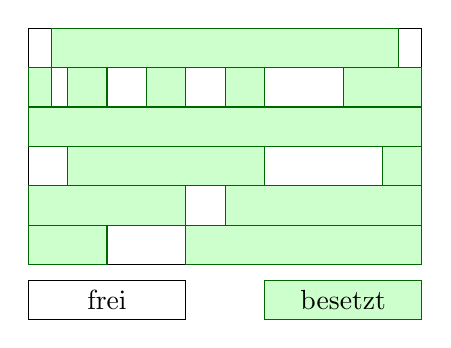
\begin{tikzpicture}
    \draw (0, 0) rectangle (5, 3) ;
    \draw (0, -0.7) rectangle (2, -0.2) node[pos=.5] {frei};
    \filldraw[fill=green!20!white, draw=green!40!black] (3, -0.7) rectangle (5, -0.2) node[pos=.5] {besetzt};
    \filldraw[fill=green!20!white, draw=green!40!black] (0,0) rectangle (1,0.5);
    \filldraw[fill=green!20!white, draw=green!40!black] (2,0) rectangle (5,0.5);
    \filldraw[fill=green!20!white, draw=green!40!black] (0,0.5) rectangle (2,1);
    \filldraw[fill=green!20!white, draw=green!40!black] (2.5,0.5) rectangle (5,1);
    \filldraw[fill=green!20!white, draw=green!40!black] (0.5,1) rectangle (3,1.5);
    \filldraw[fill=green!20!white, draw=green!40!black] (4.5,1) rectangle (5,1.5);
    \filldraw[fill=green!20!white, draw=green!40!black] (0,1.5) rectangle (5,2);
    \filldraw[fill=green!20!white, draw=green!40!black] (0,2) rectangle (0.3,2.5);
    \filldraw[fill=green!20!white, draw=green!40!black] (0.5,2) rectangle (1,2.5);
    \filldraw[fill=green!20!white, draw=green!40!black] (1.5,2) rectangle (2,2.5);
    \filldraw[fill=green!20!white, draw=green!40!black] (2.5,2) rectangle (3,2.5);
    \filldraw[fill=green!20!white, draw=green!40!black] (4,2) rectangle (5,2.5);
    \filldraw[fill=green!20!white, draw=green!40!black] (0.3,2.5) rectangle (4.7,3);
\end{tikzpicture}
 \end{minipage}\\


% Fragmentierungsproblem:\\
% \multicolumn{2}{l}{
%     \begin{minipage}
%     \begin{itemize}
%         \item tritt auf wenn während der Laufzeit new/delete gemacht wird
%         \item kann verhindert werden wenn nur beim Heruntefahren delete gemacht wird
%         \item die Speicherbeschreibung wird langsam, weil beim erneuten allozieren, zuerst ein Speicherbereich gesucht werden muss, welcher gross genug ist
%         \item es können unbrauchbare kleine Speicherbereiche entstehen
%     \end{itemize}
%     \end{minipage}
%}

\end{tabular}

Fragmentierungsproblem:
\begin{itemize}
    \item tritt auf wenn während der Laufzeit new/delete gemacht wird
    \item kann verhindert werden wenn nur beim Heruntefahren delete gemacht wird
    \item die Speicherbeschreibung wird langsam, weil beim erneuten allozieren, zuerst ein Speicherbereich gesucht werden muss, welcher gross genug ist
    \item es können unbrauchbare kleine Speicherbereiche entstehen
\end{itemize}





% \begin{compactitem}
% \item Fully Static Allocation
% \item LIFO Allocation
% \item Pool Allocation
% \item Block Allocation
% \item Region Allocation
% \end{compactitem}
\paragraph{Allocation Strategies: }~\\
\begin{tabular}{l||p{7cm}|p{7cm}|}
                        &  Fully Static Allocation & LIFO Heap Allocation\\
    \hline \hline
                        &   Daten nicht auf dem Heap $\rightarrow$ Exakte bzw. max. Anzahl der Objekte ist determinierbar. & Dynamische Allokation ausserhalb des runtime Stacks $\rightarrow$ Diese Allokationen sind immer LIFO (wie beim Stack)\\
    Speed               &   praktisch unendlich, deterministisch    & Sehr schnell, deterministisch \\
    Fragmentation       &   Nicht m"oglich                          & M"oglich, einfach zu erkennen\\
    Memory leaks        &   Nicht m"oglich                          & M"oglich, einfach zu erkennen\\
    Memory exhaustion   &   Nicht m"oglich                          & M"oglich\\
    
    
    
\end{tabular}

\vspace{1cm}

\begin{tabular}{l||p{7cm}|p{7cm}|}
                        &  Pool Allocation & Block Allocation\\
    \hline \hline       
                        & Pool Allokationen sind \textbf{alle gleich gross} (bzw. alle so gross, wie das gr"osste Element)

                        &   Verschiedene Sets von Pools mit verschiedenen Gr"ossen 
                        \newline
                        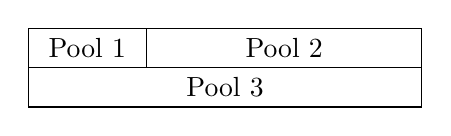
\begin{tikzpicture}
                            \draw (0, 0) rectangle (1.5, 0.5) node[pos=.5] {Pool 1};
                            \draw (1.5, 0) rectangle (5, 0.5) node[pos=.5] {Pool 2}; 
                            \draw (0, 0) rectangle (5, -0.5) node[pos=.5] {Pool 3}; 
                        \end{tikzpicture}\\
    Speed               &   Sehr schnell, deterministisch       & Schnell, praktisch deterministisch  \\
    Fragmentation       &   Nicht m"oglich                      & Nicht m"oglich\\
    Memory leaks        &   M"oglich                            & M"oglich, einfach zu erkennen\\
    Memory exhaustion   &   M"oglich                            & M"oglich\\
    
    
    
\end{tabular}
\\
% Fully Static Allocation: 
% \begin{itemize}
% \item Daten nicht auf dem Heap $\rightarrow$ Exakte bzw. max. Anzahl der Objekte ist determinierbar.
% \item \textbf{Speed}: praktisch unendlich, deterministisch
% \item \textbf{Fragmentation}: Nicht m"oglich
% \item \textbf{Memory leaks}: Nicht m"oglich
% \item \textbf{Memory exhaustion}: Nicht m"oglich
% \end{itemize}

% LIFO Heap Allocation: 
% \begin{itemize}
% \item Dynamische Allokation ausserhalb des runtime Stacks $\rightarrow$ Diese Allokationen sind immer LIFO (wie beim Stack)
% \item \textbf{Speed}: Sehr schnell, deterministisch 
% \item \textbf{Fragmentation}: M"oglich, einfach zu erkennen
% \item \textbf{Memory leaks}: M"oglich, einfach zu erkennen
% \item \textbf{Memory exhaustion}: M"oglich
% \end{itemize}

% Pool Allocation: 
% \begin{itemize}
% \item Heap Allokationen sind \textbf{alle gleich gross} (bzw. alle so gross, wie das gr"osste Element) 
% \item \textbf{Speed}: Sehr schnell, deterministisch 
% \item \textbf{Fragmentation}: Nicht m"oglich
% \item \textbf{Memory leaks}: M"oglich
% \item \textbf{Memory exhaustion}: M"oglich
% \end{itemize}

% Block Allocation: 
% \begin{itemize}
% \item Verschiedene Sets von Pools mit verschiedenen Gr"ossen 
% \item \textbf{Speed}: Schnell, praktisch deterministisch 
% \item \textbf{Fragmentation}: Nicht m"oglich
% \item \textbf{Memory leaks}: M"oglich
% \item \textbf{Memory exhaustion}: M"oglich
% \end{itemize}

\textbf{Region Allocation:} N"utzlich wenn alle Heapobjekte simultan frei gegeben werden. 
\subsection{POD (Plain Old Data)}
Folgende sind POD
\begin{itemize}
 \item alle C Datentypen (int, float, uws.)
 \item c++11 Klassen, Unions, Structs wenn folgendes nicht enthalten 
 \begin{itemize}
     \item Basisklassen
     \item Virtual Funktion
     \item Non-static data mebemrs of refence type (int\& a;)
     \item Non-static data members of non-POD(z.B. virtuelle Klasse) ( types (int a;)
 \end{itemize}
\end{itemize}
POD Typen in C++98/03 ist strikter, weil private und protected data members ausgeschlossen sind. Mit private und protected kann man das ROMable verhindern.

\subsection{C++ and ROM}
Folgendes ist ROMable: 
\begin{compactitem}


\item POD Type
\item Wert ist vor Laufzeit bekannt
\item Wert kann zur Laufzeit nicht modifiziert werden
\item Warum sind Konstanten mit \#define schlecht?
	\begin{compactitem}
		\item Sie respektieren den Scope nicht
		\item weder private noch protected
		\item kein Typ
	\end{compactitem}
	$\rightarrow$ Besser mit const. Oder noch besser mit enum (negative Zahlen auch möglich) 
\item Werden geROMt, wenn: Als const definiert, wenn sie keine mutierenden
	Daten enthalten, Wenn sie mit bekannten Werten initialisiert werden
	w"ahrend der Kompilation.
\end{compactitem}

\subsection{Schlüsselwörter und Speicher}  (Praktikum 12)
Konstanten\\
\begin{tabular}{l|l}
\hline
   \#define  & + Bei nicht Verwendug entsteht weder Code noch Daten\\
             & - keine Typenprüfung, Makroprobleme\\ 
             & pro Kompilationseinheit wird eine Speicherplatz benötigt für die Konstante \\ \hline
    const    & - Erzeugt auch Code und Daten wenn auch nicht gebraucht\\ 
             & Konstante wird nur einmal pro Projekt erzeugt\\\hline
    enum     & + Bei nicht Verwendug entsteht weder Code noch Daten\\
             & auch negative Zahlen\\\hline
\end{tabular}

\begin{lstlisting}
const char* pc1 = "Hello World"; // "Hello World" is ROMable (but pc1 is not)
const char* const pc2 = "World"; // "World" is ROMable (and may be shared with  "Hello World") pc2 is also ROMable
\end{lstlisting}
Für Integer Konstanten sollte immer enum verwendet werden. Für Double Konstanten wird empfohlen die const Variante zu wählen.\\

\begin{tabular}{l|l}
\hline
   static   & Variablen, Arrays werden auf in den Datenbereich gespeichert, nicht auf dem Stack\\
            & Variablen ausserhalb von Funktionen, sind File Globale\\
            & Variablen innerhalb von Funktionen, werden das erste Mal mit Null initialisiert\\
            &  Behalten den Wert auch wenn Out-Of-Scope\\ \hline
    const   & Daten werden ins Rom geschrieben \\
    vtbl's  & werden in den Read Only Bereich gespeichert (ROM)
\end{tabular}\\




\subsection{Modeling Memory-Mapped I/O}
Viele Systeme haben ihre I/O (\textit{memory-mapped IO devices}) im Programm-Adressbereich.
Mit C++ ist es einfach diese \textit{memory-mapped IO devices} mithilfe von Objekten anzusteuern.

\begin{tabular}{|p{9.2cm}|p{9.2cm}|}
    \hline
    Placement new   &   Ras Casts\\
    \hline \hline
    + Konstruktor wird automatisch aufgerufen & - Konstroktur muss zusätzlich aufgerufen werden \\
    - Kann zusätzlichen Overhead generieren (Kompiler abhängig) & Keinen Overhead\\ \hline
\end{tabular}

\vspace{0.5cm}

\begin{tabular}{|p{9.2cm}|p{9.2cm}|}
    \hline
    Compiler Extension     &   Linker Commands \\
    \hline\hline
    - Nicht Portabel & + Besser Portabel als Compiler Extension (Platform spezifische Adressen sind im Linkerskript vorhanden) \\
    + Kein Pointer \newline ($\rightarrow$ kein benötigter Speicher für den Pointer) & Mangled Names werden verwendet\\ 
    \hline
\end{tabular}

\paragraph{Modeling Memory-Mapped IO}
\begin{itemize}
	\item Atomic reads/writes may require explicit synchronization.
	\item Individual bits may sometimes be read-only, other times write-only.
	\item Clearing a bit may require assigning a 1 to it.
	\item One status register may control more than one data register.
		E.g., bits 0-3 are for one data register, bits 4-7 for another.	
\end{itemize}

\paragraph{Modeling a Control Register}~
\begin{lstlisting}
enum { bit0 = 0x1, bit1 = 0x2, ... , bit31 = 0x80000000 };

class ControlReg {
public:
	bool ready() const 	{ return regValue & bit0; }
	bool interruptsEnabled() const { return regValue & bit2; }
	void enableInterrupts() { regValue |= bit2; }
	void disableInterrupts(){ regValue &= ~bit2; }
private:
	volatile unsigned regValue;		// data in the register may change
									// outside program control
};
\end{lstlisting}

All functions are inline, so their existence should incur no cost.

\paragraph{Placement new vs. Raw Casts}~\\
\emph{Placement new} wird normalerweise dem \emph{raw} \texttt{reinterpret\_cast} Vorgezogen, \emph{placement new} den Konstruktor aufruft, was mit \texttt{reinterpret\_cast} selber gemacht werden müsste:
\begin{lstlisting}
pcr->ControlReg();
\end{lstlisting}

\paragraph{Placement new}~\\
Operator new’s fundamental job is not to allocate memory, it’s to identify where an object should go.

\begin{itemize}
	\item You can pass operator new where you want to put something, and it will return that location
	\item This form of operator new is called placement new.
			It’s a standard form available everywhere.
\end{itemize}

Beispiel mit Pointer:
\begin{lstlisting}
ControlReg * const pcr = new (reinterpret_cast<void*>(0xFFFF0000)) ControlReg;

while (!pcr->ready()) ; 			// wait until the ready bit is on
pcr->enableInterrupts(); 			// enable device interrupts
if (pcr->interruptsEnabled())... 	// if interrupts are enabled...

\end{lstlisting}

Beispiel mit Referenz:
\begin{lstlisting}
ControlReg& cr = *new (reinterpret_cast<void*>(0xFFFF0000)) ControlReg;

while (!cr.ready()) ; 				// wait until the ready bit is on
cr.enableInterrupts(); 				// enable device interrupts
if (cr.interruptsEnabled()) ... 	// if interrupts are enabled...
\end{lstlisting}
~ \\
Mit \textit{placement new} wird kein Speicher alloziert, somit darf auch kein delete ausgeführt werden.
\begin{lstlisting}
    int * a = new int[10];          //Speicher Allozierung 
    delete[] a;                     //Heap wird gelöscht wichtig delete[] für Array
    
    int * b = new (0xFFFF0000) int; //Placement new an der Adressse 0xFFFF0000
    delete b;                       //!!ERROR, Keine Delete beim Placement new
\end{lstlisting}

\paragraph{Raw Casts}~
\begin{lstlisting}
ControlReg *pcr = reinterpret_cast<ControlReg*>(0xFFFF0000);	// pointer version

ControlReg& cr = *reinterpret_cast<ControlReg*>(0xFFFF0000);	// reference version
\end{lstlisting}



\paragraph{Direkt vs Indirekt}~
\\
\vspace{0.5cm}
\begin{tabular}{|p{9.2cm}|p{9.2cm}|}
    \hline
    Direkt   &   Indirekt\\
    \hline \hline
    Enthalten nur statische Daten & Objekte nicht an eine spezifische Adresse gebunden (wird vom Client mit Template oder mit einem Konstruktor Argument definiert\\
    Enthalten nie virtuelle Funktionen & Kann zusätzliche Daten Member enthalten\\
    Schneller als Indirekt& Benötigt zusätzlichen Speicher (Pointer)\\
    & Flexibler als direkt\\
    \hline
\end{tabular}



\paragraph{Direkt}~
\\
\begin{tabular}{|p{9.2cm}|p{9.2cm}|}

\begin{lstlisting}
class OutputDevice3
{
  public:
    ControlReg& control() {return cr;}
    void write(uint32_t value) {data = value;}
  private:
    OutputDevice3(const OutputDevice3&); // prevent copying
    ControlReg cr;
    volatile uint32_t data;
};
\end{lstlisting}
&
Client
\begin{lstlisting}
// create OutputDevice3 object at address 0xFFFF0000
OutputDevice3& od =
*new (reinterpret_cast<void*>(0xFFFF0000)) OutputDevice3;
\end{lstlisting}
\end{tabular}

\paragraph{Indirekt}~
\\
\begin{tabular}{|p{9.2cm}|p{9.2cm}|}
\begin{lstlisting}
class OutputDevice1
{
  ...
  private:
    ControlReg* const pcr; // data members that do not map
    volatile uint32_t* const pd; // to MMIO device registers
    uint32_t lastValueWritten; // useful for write-only regs
};
\end{lstlisting}
&
Client

\\
\hline
\begin{lstlisting}
class DeviceBase {
  public:
    virtual void reset() = 0;
    ...
};

class OutputDevice1: public DeviceBase {
  public:
    virtual void reset();
    ...
};

template<uint32_t controlAddr, uint32_t dataAddr>
class OutputDevice2: public DeviceBase {
public:
virtual void reset();
...
};
\end{lstlisting}
& 
\begin{lstlisting}
OutputDevice1 od1a(0xFFFF0000, 0xFFFF0004);
OutputDevice1 od1b(0xFFFF0010, 0xFFFF0014);
...
OutputDevice2<0xEEEE0000, 0xEEEE0010> od2a;
OutputDevice2<0xEEEE0020, 0xEEEE0040> od2b;
...
DeviceBase* registers[] = {&od1a, &od1b, ..., &od2a, &od2b, ...};
const std::size_t numRegisters =
sizeof(registers)/sizeof(registers[0]);
...
for (std::size_t i = 0; i < numRegisters; ++i)
{ // reset all registers in system
  registers[i]->reset();
}
\end{lstlisting}
\end{tabular}

\paragraph{Preventing Client Errors}~

\begin{tabular}{|p{9.2cm}|p{9.2cm}|}
\begin{lstlisting}
// class modeling hardware directly
class OutputDevice3 
{ // prevents some kinds of client errors
  ...
  private:
    ~OutputDevice3() {}
    ControlReg cr;
    volatile uint32_t data;
};
\end{lstlisting}
& 
\begin{lstlisting}
OutputDevice3 d; 
// error! implicit destructor invocation.
// (We want to prevent MMIO objects from
// being placed on the stack.)

OutputDevice3* pd =
new (reinterpret_cast<void*>(0xFFFF0000)) OutputDevice3; // fine
...
delete pd; // error! another implicit destructor invocation
\end{lstlisting}
\end{tabular}
